\subsection{THE HAUSDORFF UNIFORM SPACE ASSOCIATED WITH A UNIFORM SPACE}

PROPOSITION 16. Let X be a uniform space and i the canonical mapping of X into its Hausdorff completion \(\hat{\mathbf{X}}\) . For each uniformly continuous mapping \(f\) of X into a Hausdorff uniform space Y, there is a unique uniformly continuous mapping \(h: i(\mathbf{X}) \to \mathbf{Y}\) such that \(f = h \circ i\) .

We may identify Y with a subspace of its completion \(\hat{Y}\) (no. 7, Corollary to Proposition 12), and f can then be considered as a uniformly continuous mapping of X into \(\hat{Y}\) . By virtue of Theorem 3, f is then of the form \(f = g \circ i\) , where g is a uniformly continuous mapping of \(\hat{X}\) into \(\hat{Y}\) . If h is the restriction of g to \(i(X)\) , then clearly \(f = h \circ i\) , and h maps \(i(X)\) into Y. The uniqueness of h is trivial.

The pair \((i, i(X))\) is therefore the solution of a universal mapping problem (Set Theory, Chapter IV, § 3, no. 1), where this time we take the \(\Sigma\) -sets to be Hausdorff uniform spaces, and the \(\sigma\) -morphisms (resp. \(\alpha\) -mappings) to be uniformly continuous mappings (resp. uniformly continuous mappings of X into a Hausdorff uniform space).

DEFINITION 5. The Hausdorff uniform space \(i(\mathbf{X})\) defined in the proof of Theorem 3 is called the Hausdorff uniform space associated with \(\mathbf{X}\) .

The Hausdorff completion of X is thus the completion of the Hausdorff uniform space associated with X.

COROLLARY. Let X, Y be two uniform spaces and \(X'\) , \(Y'\) the associated Hausdorff spaces. For each uniformly continuous mapping \(f: X \to Y\) there is a unique uniformly continuous mapping \(f': X' \to Y'\) for which the diagram

\pandocbounded{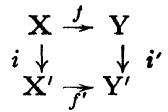
\includegraphics[keepaspectratio]{images/part002_3c8eaa6f.jpg}}

is commutative, where \(i\) and \(i'\) are the canonical mappings.

Apply Proposition 16 to \(i' \circ f: \mathbf{X} \to \mathbf{Y}'\) .

The Hausdorff space associated with a uniform space may also be characterized by the following property:

PROPOSITION 17. Let X be a uniform space, \(i(X)\) its associated Hausdorff space, and let \(f\) be a mapping of X onto a Hausdorff uniform space \(X'\) , such that the uniformity of X is the inverse image under \(f\) of the uniformity of \(X'\) . Then the mapping \(g:i(X)\to X'\) such that \(f=g\circ i\) is an isomorphism.

By Proposition 16, g is uniformly continuous; also g is obviously surjective, and is also injective because the relation \(f(x) = f(y)\) implies by definition that \((x,y)\) belongs to all the entourages of X, and therefore that \(i(x)=i(y)\) (no. 7, Proposition 12). Finally, the entourages of \(X'\) are the images under \(f\times f\) of the entourages of X (§ 2, no. 4, Remark), hence they are also the images under \(g\times g\) of the entourages of \(i(\mathbf{X})\) (no. 7, Proposition 12); hence the result.

Remark. Let R be the equivalence relation \(i(x) = i(x')\) on X. We have seen (no. 7, Proposition 12) that the graph C of R is the intersection of all the entourages of X. It is clear that every open set (and therefore also every closed set) in X is saturated with respect to R; taking account of the definition of the inverse image of a topology, we conclude that the canonical bijection of the quotient space X/R onto \(i(X)\) induced by \(i\) is a homeomorphism. The Hausdorff space associated with X can therefore be identified, qua topological space, with X/R. The canonical mapping \(i: X \to i(X)\) is open and closed, and even proper (Chapter I, § 10, no. 2, Example).

Let \(X'\) be another uniform space, \(C'\) the intersection of all the entourages of \(X'\) , and \(R'\) the equivalence relation whose graph is \(C'\) . Let \(f: X \to X'\) be a continuous mapping. Since the inverse image under \(f\) of any neighbourhood of \(f(x)\) is a neighbourhood of \(x\) , it follows that the inverse image under \(f\) of \(C'(f(x))\) contains \(C(x)\) , and therefore \(f\) is compatible with \(R\) and \(R'\) , and induces a continuous mapping \(X/R \to X'/R'\) (Chapter I, § 3, no. 4, Corollary to Proposition 6). This generalizes the corollary to Proposition 16.

